\chapter{Raw Distributions of RTT Measurements}
\label{app:rtt}

We plot in \cref{fig:rtt-count} the raw distributions of \acrshort{rtt} delays measured in
\cref{chp:doa}. As already mentioned, the \acrshort{rtt} measurements for the ``Bypass servers''
configuration can be approximated by a single-mode Gaussian distribution, with small standard
deviation and negligible outliers. Such a clean distribution is an indicator of the stable
performance of the real-world classical network used in our experiments and of the fairly constant
traffic on such network. On the other hand, measurements for the ``No \acrshort{mac}'' and
``\acrshort{poly}'' configurations are better approximated by bimodal Gaussian distributions, with
negligible differences in mean and variance of each mode across the two configurations. These more
stark variations in \acrshort{rtt} for these two configurations are most likely to be attributed to
some caching behavior in the packet processing pipeline. Nevertheless, the overall mean
\acrshort{rtt} for each configuration is approximately equal to the mean of the strongest mode. The
following tables report mean and standard deviation for all configurations, and for all modes of the
distributions --- where these are bimodal.
% --- for payload sizes of \num{12} bytes (\cref{tab:app-rtt-pl-12}) and \num{1200} bytes
%  (\cref{tab:app-rtt-pl-1200}).

\begin{table}[h]
    \begin{tabularx}{\linewidth}{@{} lrYYYY @{}}
        \toprule
        \textbf{Server}                    &                & \multicolumn{2}{c}{\textbf{\acrshort{rtt} mean} [\unit{\us}]} & \multicolumn{2}{c}{\textbf{\acrshort{rtt} std} [\unit{\us}]} \\
        \cmidrule(l){3-4}
        \cmidrule(l){5-6}
        \textbf{configuration}             & \textbf{Scope} & \textbf{Pl. 12}     & \textbf{Pl. 1200}                       & \textbf{Pl. 12}     & \textbf{Pl. 1200}                      \\
        \midrule
        Bypass servers                     & Overall        & \num{3657}          & \num{3881}                              & \num{23}            & \num{22}                               \\
        \midrule                                                                                                                                              
        \multirow{3}{*}{No \acrshort{mac}} & Overall        & \num{13821}         & \num{13993}                             & \num{3142}          & \num{2876}                             \\
                                           & First mode     & \num{14036}         & \num{14089}                             & \num{797}           & \num{767}                              \\
                                           & Second mode    & \num{11251}         & \num{11400}                             & \num{446}           & \num{397}                              \\
        \midrule                                                                                                                                              
        \multirow{3}{*}{\acrshort{poly}}   & Overall        & \num{14387}         & \num{13959}                             & \num{5044}          & \num{2867}                             \\
                                           & First mode     & \num{14099}         & \num{14015}                             & \num{861}           & \num{729}                              \\
                                           & Second mode    & \num{11300}         & \num{11442}                             & \num{398}           & \num{356}                              \\
        \bottomrule
    \end{tabularx}
    \caption{
        Mean and standard deviation of \acrshort{rtt} for different configurations of the
        \acrshort{doa} servers and for all modes of the analyzed distributions, for payloads of
        \num{12} bytes (Pl. 12) and \num{1200} bytes (Pl. 1200).
    }
    \label{tab:app-rtt}
\end{table}

\begin{figure} \centering
    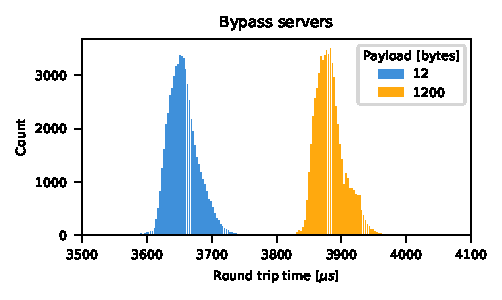
\includegraphics[width=0.6\linewidth]{figures/rtt-distribution-no-proxy.pdf}
    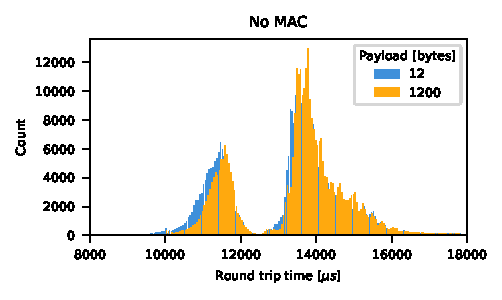
\includegraphics[width=0.6\linewidth]{figures/rtt-distribution-no-mac.pdf}
    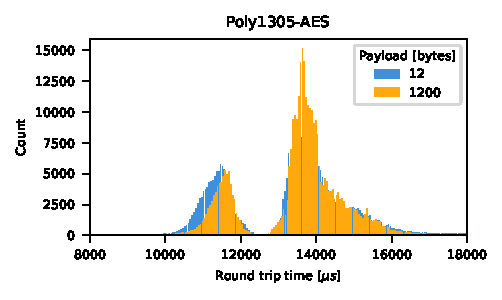
\includegraphics[width=0.6\linewidth]{figures/rtt-distribution-poly1305.pdf} \caption{
        Distribution of \acrshort{rtt} measurements for the ``Bypass servers'', ``No
\acrshort{mac}'' and ``\acrshort{poly}'' configurations, for message payloads of \num{12} and
\num{1200} bytes. Each histogram consists of 200 bins. } \label{fig:rtt-count} \end{figure}
